%!TEX root =../../thesis-ex.tex

\chapter{Assisting Business Decision Making with Natural Language to SQL Interface}
\label{ch5:nl2sql}

With the large penetration rate of mobile devices and gradually increasing market of mobile business intelligence, mobile data analysis tools such as Microsoft Power BI and Google Analytics has been popular among data analysts, allowing hundreds of millions of business users to analyze their data on the go. A convenient feature on these platforms is the natural language interface (NLI) feature, which allows mobile users to query the database in natural language sentences. 

There exists a long history of research on translating natural language to database queries. Following the business intelligence services, in recent years, an increasing interests are on cross-domain translation with a large number of database schemas. In this section, we study the problem of cross-domain complex query translation, where schemas in the training fold, development fold, and testing fold are disjoint. We build our method on top of the current state-of-the-art text-to-SQL model named IRNet~\cite{guo2019towards}. By leveraging the value items in the database that match the natural language question, we achieve an exact matching accuracy of 68.2\%, 2.7\% higher than the that of IRNet (65.5\%). Then we conduct an analysis on the remaining errors and propose ideas on further improving the accuracy. 

\section{Introduction}

Recent years have witnessed great attention in the problem translating a natural language question to an SQL statement. By providing a natural language interface, users can easily query the database by typing a natural language questions. Natural language interface to database queries is frequently seen in business intelligence applications (e.g., Microsoft Power BI). An example of such interface is displayed in Figure~\ref{ch5:fig1:powerbi1}, where the user can type a natural language query in the ``question'' box, during this process the system interactively display the execution results of the translated SQL statement. The same feature has also been deployed on the corresponding app on mobile devices. The natural language interface feature has been well received from users. From one review for the mobile application of Google Analytics, one user commented: \emph{the best feature perhaps is the natural language query and it gives you the required report}. 

\begin{figure}[h]
\centering
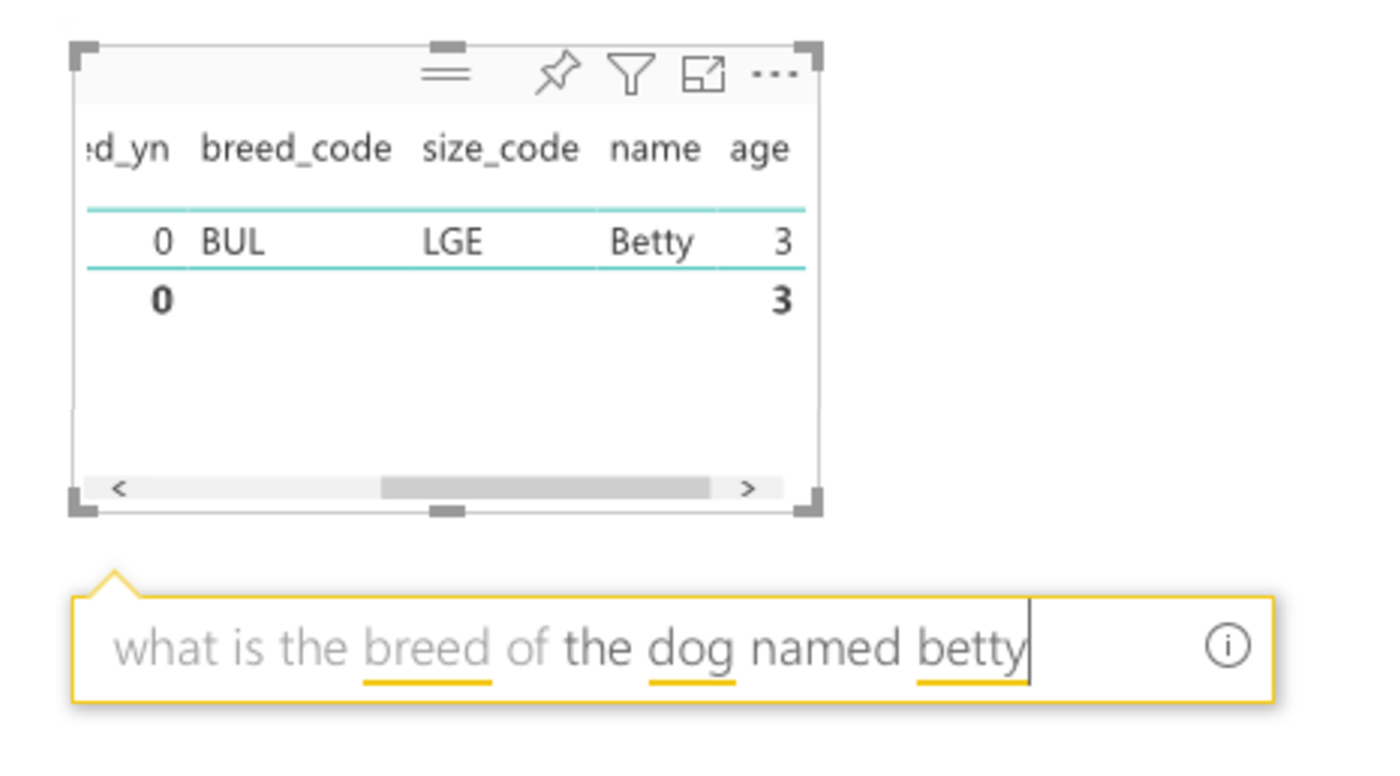
\includegraphics[width=.5\textwidth]{figure/chapter1/powerbi1_crop}
\caption{A snapshot of Microsoft Power BI\label{ch5:fig1:powerbi1}}
\end{figure}

The problem of mapping a natural language question to a database query has been a long-standing problem, attracting attentions from multiple communities. The topic was studies in the 1970s, e.g., the Precise system~\cite{popescu2003towards}. In the past, however, most of the focuses were on building the interface with the same schema. For example, one of the datasets contain questions users could ask within a flight booking system. Therefore, the trained NLI usually cannot generalize to other schemas. Such NLI can usually achieve a good performance by practicing the following steps: first, enumerating potential SQL statement within the database; second, for each SQL statement, translating the SQL statement to its corresponding natural language question; third, for each natural language question, use crowd sourcing to obtain a large number of its paraphrased question, e.g., by replacing words with synonyms, or by restructuring the sentence. Because the problem is within a closed domain, there is usually a limited number of questions that the user can ask, allowing models to achieve good performances. 

With the new business intelligence tools, however, it is quite clear that it is no longer enough for the NLI to only be able to answer questions within one schema, because it should be expected that user questions come from a new schema that is not seen in the training data. The problem of translating natural language to SQL statement, but also generalizing to unseen domains have been a trending topic in recent years. Multiple large-scale datasets are released since 2017, new results are published on arxiv in a monthly base. In these datasets, the schemas in the training fold and testing fold are fully separated, e.g., the Spider dataset contains 145 schemas in the training fold and 20 schemas in the development fold. 

The Spider dataset is the larges cross-domain dataset that contains the most complex SQL structures. An earlier dataset, WikiSQL, contains 80K questions from 24K database schemas. However, this dataset is over-simplified. Each schema contains only 1 table, and all the questions come from the same template, i.e., \texttt{SELECT (agg\_func(column))+ FROM table WHERE (agg\_func(column) operator value)+}. As a result, the trained NLI does not have the ability to tell important information such as whether a \texttt{WHERE} condition is included in the question (it just assumes it does). The Spider dataset, on the other hand, contain more complex queries. It not only include queries which both include and does not include there \texttt{WHERE} statement, but also other SQL keywords such as \texttt{GROUP BY, HAVING} and nested queries. 

As a result, in this work, we explore how to improve the performance of natural language to SQL prediction on the Spider dataset. State-of-the-art approaches achieve approximately 64\% exact matching accuracy~\cite{guo2019towards}. To improve the performance, we first need to identify the deficiency of the current model. A major challenge in Spider is to how predict the columns correctly~\cite{yu2018syntaxsqlnet}:

\begin{enumerate}
\item \texttt{Give the flight numbers of flights landing at APG}
\item \texttt{What is the last name of the student who has a cat that is 3 year old}
\end{enumerate}

In the first example, the correct SQL statement is \texttt{SELECT flightNo from Flights WHERE DestAirport = APG}. However, in one of previous results~\cite{yu2018syntaxsqlnet}, the column DestAirport has been wrongly predicted as FlightNo. In the second example, the correct statement is \texttt{SELECT T1.lname FROM student AS T1 JOIN has\_pet AS T2 ON T1.stuid  =  T2.stuid JOIN pets AS T3 ON T3.petid  =  T2.petid WHERE T3.pet\_age  =  3 AND T3.pettype  =  'cat'}. However, the column \texttt{pet\_age} is often wrongly predicted as the age of the student. 

Intuitively, the column prediction results can benefit from knowing the column value. In the first example, if we know that APG must be the name or the abbreviation of an airport, it is less likely to wrongly select the column FlightNo. In the second example, if we know that student ages are usually larger than 3, it is more likely to weight pet\_age more than student\_age. 

In other words, being aware of the column values can help us better predict columns. The values in database tables are often often named entities, or numbers. Such values are usually more distinguishable than the column value names and table names, when human reads the natural language question, the first thing to notice is also often the named entity values in the sentences. Given the input sentence, if we can know A. what values it mentions, and B. which columns contain these values, intuitively it should help improve the column predictor by avoiding the mistakes in the above two examples. 

First, we can reduce the question to a simpler question:

RQ1. If we knew both A and B perfectly, how much does it help with improving the state-of-the-art result on Spider?

We conduct experiments by injecting the ground truth column values to the state-of-the-art approach IRNet~\cite{guo2019towards} and observe 3.5\% increase in the exact matching accuracy (from 65.5\% to 69\%) in the development accuracy. In reality, however, we do not know the the ground truth column values in the development fold. One easier approach for obtaining such values is to match the database cells against the natural language question. 

RQ2. If we can have access to the database values, how much does it help in improving the state-of-the-art results?

To answer this question, we develop a rule-based keywords matcher to find the potentially matched values. The matcher can achieve 94\% recall, but it contains many false positive results, especially when the database is larger. For example, in the database wta\_1, the question \texttt{What is the name of the winner who has won the most matches and how many rank point does this player have?} was matched by the column \texttt{person LastName} and value \texttt{won}. To remove these false positive results, we develop another rule-based module for post-processing the matcher result. For example, in this example, our module can detect that the column name \texttt{person LastName} appears as the subject of the questioning word \emph{what}, therefore it should appear after SELECT instead of WHERE, therefore we remove the column. The post-processing finally achieves 93.6\% accuracy, and 1.9\% false positive rate. Notice that some databases are absent in the dataset, in those cases it is impossible to achieve 100\% accuracy. After injecting the column values found by our rule-based matcher, we observe 2.7\% increase in the exact matching accuracy (68.2\%). A complete description of the modules in our rule-based matcher is described in Section~\ref{sec:rule}. 

After answering the two questions, we ask one question: what mistakes does IRNet make in the remaining 32.8\% erroneous cases? If we can achieve close to 100\% accuracy in column matching, how much overall accuracy does it make? What are the most frequent mistakes? To answer this question, we conduct an empirical study in Section~\ref{sec:study}. 

%!TEX root =../../thesis-ex.tex

\section{Related Work}
\label{sec:relwork}

The task of Natural Language Interface to Database (NLIDB) has received significant attention since the 1970s \cite{warren1982efficient,androutsopoulos1993masque,popescu2003towards,hallett2006generic}. Most of the early work focuses on the case where there is only one database being asked. For example, the famous ATIS dataset consists of 4,978 questions for the airline booking system. The Geo dataset consists of 880 questions on geographic facts, e.g., \emph{give me the cities in virginia}. These datasets are frequently used in existing work on natural language interface. It is therefore difficult to adapt such trained NLI to new domains, because with new database schemas, the relations will be different. 

Recently, more and more work has been focusing on the cross-domain scenario, including two large dataset Overnight~\cite{wang2015building} WikiSQL~\cite{zhong2017seq2sql} and Spider~\cite{yu2018spider}. The scale: the first dataset, Overnight consists of only 8 domains, each domain consists of close to 1K utterance; WikiSQL consists of the largest number of utterances and schemas. Way of construction: all three datasets are constructed using crowd sourcing, the difficulty of constructing a dataset is that the utterance and SQL statement must alight correctly. To achieve a large scale, the three datasets use difference strategies: Overnight leverage an alignment of natural language and SQL templates, e.g., \texttt{whose COLUMN (>|<|=...) VALUE} is the natural language template that corresponds to \texttt{WHERE COLUMN (>|<|=...) VALUE}. It first recursively automatically construct more complex templates based on rules in these templates. Then they enumerate compatible column names and value names for replacing \texttt{COLUMN} and \texttt{VALUE} in both template, and ask human to rephrase the natural language question for as many different versions as possible. In Overnight, each domain has its own training and testing fold, so the learner does not need to be able to adapt to new domain, but can learn the general grammar from the shared templates. 

Slightly different than overnight, WikiSQL first introduced the scenario where each database schema has just a few utterance, but there are 24K different schemas. It is possible that such scenario is inspired by the business intelligence need, where each customer may just ask a few questions to their uploaded database tables, but there can be a large number of such customers whose data can be used for training. It also introduce the scenario where the training schema and the testing schema are completely separated. An interesting question is what has been learned from the completely different schemas. A previous paper studies the domain adaptation and found a good performance~\cite{dadashkarimi2018zero}. 

WikiSQL is the largest dataset, but the sketch oversimplies the difficult question of NL2SQL. Because the database extracted from Wikipedia are more noisy, it may be more difficult to construct more complex queries. The dataset consists of only \texttt{SELECT} and \texttt{WHERE}, such queries can be randomly sampled from any table without a lot of constraint on the correctness, however, by randomly generated adding a set of columns to the same statement, the resulting statement might not be that meaningful. 

Spider is the latest large-scale dataset on NL2SQL. Different from WikiSQL, the dataset in Spider are pooled from multiple resources, including text book databases and the existing databases for single-domain NL2SQL tasks (e.g., Geo, ATIS, Yelp). The labeling jobs are done by a number of computer science students who are good at SQL, the natural language sentences are also manually created so the sentences look more natural. They rephrase each question a few times. 

After WikiSQL and Spider came out, the topic of NL2SQL has drawn quote some attentions. State-of-the-art has achieved 86\% accuracy on WikiSQL. Some of the ideas for improving WikiSQL include using the execution result as the feedback in reinforcement learning loop~\cite{zhong2017seq2sql}, leveraging a sketch~\cite{xu2017sqlnet}, first generating a sketch then fill the missing details~\cite{dong2018coarse}, column type~\cite{yu2018typesql}, using BERT to represent utterance and column names~\cite{hwang2019achieving}, and execution-guided decoding~\cite{wang2018execution}. In the Spider dataset, the state-of-the-art model is IRNet plus BERT~\cite{guo2019towards} achieving 64\% accuracy, other works include gated graph neural network~\cite{bogin2019representing}. 

Other work on natural language interface include translating the natural language utterance to the canonical natural language template, so that the template can directly be mapped to the corresponding SQL template~\cite{su2017cross}. The study this problem on the Overnight dataset, where they apply the word analogy property of word embedding to translate the utterance, e.g., in sentence \texttt{In which seasons did Kobe Bryant play for the Lakers?} and \texttt{When did Alice start working for Mckinsey?}, how \texttt{Kobe Bryant} to \texttt{Lakers} is analogous to how \texttt{Alice} is to \texttt{Mckinsey}. Such parallelism helps explain how sentence paradigms are being learned across different domains. Another work from the programming language community \cite{yaghmazadeh2017sqlizer} has used program repair and type system, where they initially leverage a general semantic parser, then the type of columns are checked against column values, if the two types are inconsistent, they use program repair techniques to fix the statement by enumerating the potentially correct column/values. 


%!TEX root =../../thesis-ex.tex

\section{Problem Formulation}

The input of text-to-SQL contains the following components: a natural language question, a database schema that consists of one or more tables. For each table, the table name and a list of column names are also in the input. 

The problem we study in this work is: given the natural language question, table names and column names, how can we most accurately extract the column and the values that are mentioned in the target SQL question? 

The performance of column value matcher is evaluated by both accuracy and recall. The accuracy is the number of testing examples where the matched column value set containing values is the same as the ground truth column set containing values. In Spider, about 52\% examples mention at least one a column value. To achieve a good accuracy, the matcher should predict empty if no value is mentioned. 

\section{Rule-Based Matcher}
\label{sec:rule}

As there exist a trade-off between precision and recall, we use the following strategy for the matcher: first, we build a module with high recall by including any case that could be a match; second, among the result found in the first step, build a classifier for filtering out the incorrect cases. 

\subsection{First Step: Improving the Recall}

To improve the recall, we need to reduce the false negative cases, i.e., the cases which should be matched but are not matched. There are two types of false negatives: string and number. Matching string is easier than matching numbers, because string values are usually copied in the question, while numbers may be mentioned differently. The reason is that many questions contain comparison between numbers, e.g., \texttt{how many department heads are older than 56?} It is possible, however, the column \texttt{age} does not contain a value which equals 56. To improve the recall, if a question contain a number, we extract all the columns whose values are numbers. For those columns, we keep the values whose scale is closest to any numbers mentioned in the input. 

Meanwhile, sometimes the column that contain the value is \texttt{*}, e.g., for question \texttt{Which airline have less than 200 flight?} the SQL statement is \texttt{SELECT Airline FROM AIRLINES JOIN Flights HAVING count(*) < 200}. We include the column \texttt{*} if the natural language question mentions statements contains comparative statement. 

The recall of this step is 94\%.

\subsection{Second Step: Improving the Accuracy}

The main idea of improving the accuracy in the first step is to compare between columns and eliminate the columns that matches less than other columns. Due to the dependency between table names, column names and values, it is difficult to find a unified criterion in deciding whether a column should be removed or not. Still consider the above example of selecting the column \texttt{*}. When the question asks \texttt{Which airline have less than 200 flights?}, our first step includes the column \texttt{*}. Meanwhile, there may exist another column called \texttt{flight number} containing a value 200, it is also included in our first step. Since there is only 1 number in the question, which column between \texttt{*} and \texttt{flight number} should we select? The answer may not always be \texttt{*}, because if the column \text{flight number} is \text{flight count} the correct SQL statement may be \texttt{count(flight number) < 200}. 

To capture the dependency between columns, we compare similar columns and eliminate those which \emph{match less than} at least one of existing columns. Here the definition of \emph{match less} is:

\textbf{Definition}. Given two column-value pairs \texttt{(col1, val1)} and \texttt{(col2, val2)}, if pair 1 better matches the sentence than pair 2 in both the column and value, we say pair 2 \emph{matches less} than pair 1. 

The following rules capture how a column/value better matches a sentence than another column/value.

\begin{enumerate}
\item If \texttt{col1} is mentioned in the sentence while \texttt{col2} is not mentioned, \texttt{col1} matches better than \texttt{col2};
\item If \texttt{val2} is a substring of \texttt{val1}, \texttt{val1} matches better than \texttt{val2};
\item If both \texttt{val1} and \texttt{val2} are numbers, and \texttt{val1} is closer to the mentioned numbers in the sentence than \texttt{val2}, \texttt{val1} matches better than \texttt{val2}; 
\item If and the average distance from words in \texttt{col1} to the target value in the sentence are shorter than that from \texttt{col2}, pair 2 matches less than pair 1;
\item If \texttt{val1} and \texttt{val2} are equal numbers, and val1's number type matches val2's number type better, \texttt{val1} matches better than \texttt{val2}, here a number type can be age, year, quantity, etc.
\end{enumerate}

For examples, in the question \texttt{Find number of pet owned by student who are older than 20}, pair 1 = (student age, 20), pair 2 = (pet age, 3), pair 1 matches more than pair 2, because by rule 3, 20 is closer to 20 than 3, and by rule 4, the average distance of \emph{student age} to 20 is shorter than \emph{pet age} to 20. 

We implement the rules using 900 LOC, the above rules achieve an accuracy of 92\% and false positive rate of 2.7\% on the development fold of Spider.

\textbf{Discussion: Pros and Cons of using rule-based approach}. The rule-based approach is created mostly based on our observation for the output of the first step. Therefore, it is less general than, e.g., neural network approach. However, an advantage of rule-based approach is that we do not need to select the number of columns in the output. On the other hand, due to the dependency between columns, neural network approach works better under the ranking setting (than the prediction setting), and we still need to select the number of columns. 
%!TEX root =../../thesis-ex.tex

\section{Background on IRNet and Experimental Results}
\label{sec:exp}

IRNet is currently the state-of-the-art model on Spider. The main idea of IRNet is to use an intermediate representation which captures the target SQL statement. IRNet consists of 11 actions, representing the grammar rules in SQL. For each action, IRNet builds a classifier to select from a list of action values, e.g., \{UNION, INTERSECTION, NONE, EXCEPT\}. Most of the actions contains a small number of options, except for the column and table predictor. For column predictor, IRNet uses a pointer net which select from all the columns in the table. 

IRNet's column prediction result is significantly improved by leveraging BERT, mainly in the column and table prediction results. However, the result still has less than 65\% accuracy in the column prediction for the \texttt{WHERE} statements. For example, given the question \texttt{Find number of pet owned by student who are older than 20}, IRNet selects the column pet\_age instead of student\_age. To further improve the column prediction results, IRNet leverages a second external column predictor to select a ranked list of columns that are most likely the column results. It then use the top $k+1$ columns as the candidate, where $k$ is the number of columns in the ground truth. When training IRNet, the column predictor select only from the $k + 1$ columns. 

If the external column predictor can achieve 100\% accuracy, IRNet will not select a column that is not mentioned in the ground truth, as a result, it is critical to improve the results of the column predictor. 

\textbf{Adding column values to IRNet}. After extracting columns with the column matcher, we insert the column values to IRNet + BERT simply by appending the value to the end of the column names, e.g., for the question \texttt{Find number of pet owned by student who are older than 20}, the column \texttt{age} becomes \texttt{age 20} and table \texttt{student} becomes \texttt{student age 20}. 

The external column predictor achieves 80.4\% accuracy, if not leveraging the values. This column predictor gives rise to a 64\% accuracy in the exact matching result of IRNet. Here the accuracy is defined by the proportion of examples where the predicted column set exactly matches the ground truth column set. By leveraging values, we are able to achieve a 85.9\% accuracy in the external column predictor and a 68.2\% accuracy in the IRNet result. 

A question here is which column values to add to the training data. Because in the training set, we do have access to the ground truth, we can add either the ground truth column values or the matched column values (although when testing we can only add the predicted column values). We find that it works better if we add the ground truth column values to the training data. Meanwhile, we also test some simple data augmentation: for each training question, if it contains at least a column value, we add two copies of the question, first the one with the column value, second the one without the column value. We hope that this approach could help so that if the column value matcher misses a value in the test example, it can still learn from the training data without the values. However, we have not observed significant improvement. 
%!TEX root =../../thesis-ex.tex

\section{An Empirical Study on IRNet Performance}
\label{ch5:sec:study}

After achieving 68.2\% accuracy, we move on to study how to further improve the performance. Text-to-SQL is a complex problem whose accuracy relies on multiple modules. Despite the fact that there is a large gap due to the column mismatch, we ask the question: if the columns are perfectly matched, does that make the performance close to 100\%? 

To answer this question, we first pretend the external column selector can select exactly the ground truth column set, so that IRNet will not have false positive column predictions. Our experiment shows that by doing so, IRNet achieves a 72.4\% accuracy, which means even if the external column predictor is 100\% correct, there is still a 27.6\% gap towards 100\% accuracy. 

% We find that the remaining erroneous cases can be categorized into two categories: first, the sketch is predicted correctly, but some column predictions or table predictions are incorrect; second, the sketch is predicted incorrectly. We separate the two cases using one criterion: whether the rule label sequence of prediction equals that of ground truth. 

% \textbf{Not Equal:} there are 14\% cases where the sequence lengths are not equivalent. 3.5\% are due to wrong IUEN prediction (\texttt{UNION, EXCEPT, INTERSECTION}), 6.2\% are cause by the wrong prediction of Filter; 2.3\% are cause by a wrong prediction in the column number; 1.6\% are cause by the mistakes in superlative (i.e., \texttt{DESC LIMIT}).

% \textbf{Equal:} there are 13\% cases where the sequence lengths are equivalent. 5.4\% are caused by a wrong table prediction, 5.05\% are cause by a wrong aggregation prediction, 1.9\% are caused by a wrong column predictor. 

If we have access to a perfect external column selector, does that make the column selection 100\% correct? Our experiment shows this is not the case. There still exist 11\% cases where the column predictor inside IRNet would miss cases. For example:

\texttt{Example 1. How much does the most recent treatment cost?}

In the above example, the correct SQL statement is \texttt{SELECT cost\_of\_treatment FROM Treatments ORDER BY date\_of\_treatment DESC LIMIT 1}, therefore the correct column set is \texttt{cost\_of\_treatment} and \texttt{date\_of\_treatment}; however the prediction selects only \texttt{cost\_of\_treatment}. However, the question contains a word \texttt{recent}, which means there has to be a column or table that represents the time. If non of the columns predicted indicate time, there must be something missing and therefore the SQL statement is incorrect. 

This result shows that even after leveraging BERT and allowing it to choose from a perfect external column predictor, IRNet still make a significant number of mistakes in the column selection results. The fact that BERT can contextually represent the model does not mean it will always succeed in SQL prediction. The pretrained BERT containing only 30K vocabularies may have been not powerful enough to adapt to the specific domains in the schemas. For example, one of the questions is \texttt{How many students' sex are M?} where the \texttt{M} stands for \texttt{Male}. Without further information, it is difficult to make that inference. 

\section{Plans for Future Work}
\label{sec:rq3}

Given the analysis in Section~\ref{ch5:sec:study}, we plan to by explore the problem of how to increase the recall of column prediction if we allow IRNet to have a perfect external column predictor. For example, one idea is to check whether all words in a sentence have been included in the column prediction. We make the following hypothesis:

\textbf{Hypothesis 1}. If a column is mentioned in the question, it must exist in the SQL statement;

\textbf{Hypothesis 2}. If a column is mentioned in the SQL statement, it must have been mentioned either explicitly or implicitly in the question. 

For example, the observation above that identifies a missing word \texttt{treatment} would be detected as an error case based on Hypothesis 1. We can keep track of all the words in a sentence and mask those words that have already been selected, once the column selector is done, we observe the sentence and see whether some words are missing. Such signals can be leveraged as feedback to a reinforcement loop like in \cite{zhong2017seq2sql}. 